\documentclass{article}
\title{Trabajo final IFC}
\author{Ignacio Loaiza   41205127-2}
\date{04/Dic/2013}
\usepackage{graphicx}
\usepackage[left=3cm, right=3cm, top=2.5cm, bottom=2.5cm]{geometry}
\usepackage[spanish]{babel}
\begin{document}
\begin{titlepage}

\newcommand{\HRule}{\rule{\linewidth}{0.5mm}}
\center 
 
\textsc{\LARGE UNIVERSIDAD NACIONAL AUT\'ONOMA DE M\'EXICO}\\[1.5cm] 
\textsc{\Large Facultad de Ciencias}\\[0.5cm] 
\textsc{\large Laboratorio de electr\'onica}\\[0.5cm] 
\HRule \\[0.4cm]
{ \huge \bfseries Pr\'actica I: La Ley de Ohm}\\[0.4cm]
\HRule \\[1.5cm]
\begin{minipage}{0.4\textwidth}
\begin{flushleft} \large
\emph{Alumno:}\\
Ignacio \textsc{Loaiza}
\end{flushleft}
\end{minipage}
~
\begin{minipage}{0.4\textwidth}
\begin{flushright} \large
\emph{Profesor} \\
Dr. Jos\'e\ Manuel \textsc{Alvarado Reyes}
\end{flushright}
\end{minipage}\\[3cm]
{\large 19 de Agosto de 2014}\\[0.5cm]
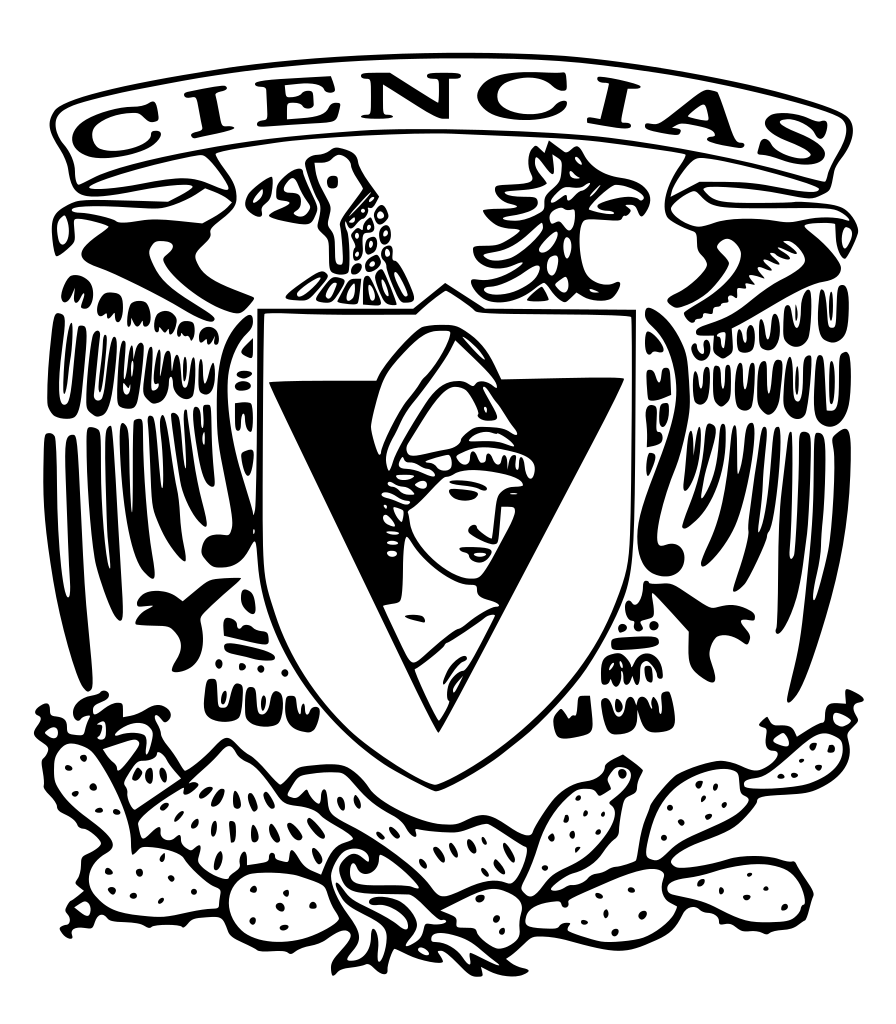
\includegraphics[width=6cm]{/home/nacho/Escuela/ciencias.png}\\[1cm]
\vfill
\end{titlepage}
\section{Resumen}
En esta pr\'actica se midieron los voltajes y corrientes en un circuito con varias resistencias en serie y en paralelo. Se busc\'o\, adem\'as de verificar la Ley de Ohm, familiarizarse con el concepto de resistencia, as\'i\ como aprender a reducir varias resistencias a una sola resistencia equivalente y aplicar las leyes de Kirchhoff.

\section{Introducci\'on}
Muchas veces, a o largo de la carrera, hemos hecho circuitos con varias resistencias \textit{en paralelo} o \textit{en serie} sin realmente saber porqu\'e\ se est\'an colocando las resistencias de esta forma. En esta pr\'actica se busca entonces conocer c\'omo var\'ian las resistencias cuando se tienen distintos tipos de arreglos, para poder as\'i\ realmente entender y hasta planear circuitos electr\'onicos.

\section{Marco Te\'orico}
Sea un circuito con una resistencia $R$ el cual es sometido a un voltaje de $V$ con una corriente $I$, se tiene entonces que, seg\'un la Ley de Ohm:
\begin{equation}
V=RI
\end{equation}
La ley de las mallas de Kirchhoff nos dice que, en una malla, se tiene que:
\begin{equation}
\sum V_i=0
\end{equation}
D\'onde $V_i$ son los voltajes que se tienen en una malla. \\ 
Para aplicar esta ley no hay que olvidar los sentidos distintos que tiene un voltaje (por lo general se toman en un sentido los voltajes de los elementos que dan corriente y en otro sentido de los que la reciben). La ley tambi\'en se puede reescribir entonces como:
\begin{equation}
\sum V_G=\sum V_R
\end{equation}
D\'onde $V_G$ son los elementos que generan la corriente y $V_R$ los que la reciben.
Se puede ver un esquema de la ley en la siguiente figura:
\begin{center}
\includegraphics[width=4cm]{malla.png}
\end{center}
\begin{center}
Figura 1: Esquema de la ley de las mallas.
\end{center}

La ley de los nodos de Kirchhoff dice que, en un nodo:
\begin{equation}
\sum I_i=0
\end{equation}
D\'onde $I_i$ son las intensidades de la corriente que se tienen en un nodo. Esta ley tambi\'en se puede escribir como:
\begin{equation}
\sum I_E=\sum I_S
\end{equation}
D\'onde $I_E$ son las corrientes entrantes al nodo y $I_S$ son las salientes.
Se puede ver un esquema de esta ley en la siguiente figura:
\vspace{5cm}
\begin{center}
Figura 2: Esquema de la ley de los nodos.
\end{center}

Sean $n$ resistencias en serie, se tiene que se puede reducir este sistema a una resistencia equivalente con la siguiente f\'ormula:
\begin{equation}
R_{eq}=\sum _n R_n
\end{equation}
Se puede ver el arreglo en serie en el siguiente esquema:
\begin{center}
\includegraphics[width=2cm]{serie.png}
\end{center}

\begin{center}
Figura 3: Esquema de resistencias en serie.
\end{center}
Sean $n$ resistencias en paralelo, se tiene que se puede reducir este sistema a una resistencia equivalente con la siguiente f\'ormula:
\begin{equation}
R_{eq}=\Big( \sum_n (R_n)^{-1} \Big) ^{-1}
\end{equation}
Se puede ver el arreglo en paralelo en el siguiente esquema:
\begin{center}
\includegraphics[width=8cm]{paralelo.png}
\end{center}
\begin{center}
Figura 4: Esquema de resistencias en paralelo.
\end{center}
Cabe notar que, de estas leyes, se justifica que se debe de conectar el mult\'imetro en serie para medir corrientes (ya que no hay ning\'un nodo se tiene la misma corriente) y en paralelo para medir voltajes (se tiene una peque\~na malla entre el mult\'imetro y el elemento al cual se le est\'a\ midiendo el voltaje, teniendo voltajes iguales).



\section{Experimentaci\'on}
\subsection{Materiales}
Los materiales utilizados en esta pr\'actica fueron:
\begin{enumerate}
\item Fuente de voltaje continuo variable
\item Resistencias de: $1.2k\Omega$, $4.7 k\Omega$ y $2\Omega$
\item Mult\'imetro digital
\end{enumerate}

\subsection{M\'etodo experimental}
Se hizo el circuito c\'omo se ve a continuaci\'on:
\begin{center}
\includegraphics[width=10cm]{circuito.png}
\end{center}
\begin{center}
Figura 5: Esquema del circuito experimental
\end{center}
D\'onde $R_1=R_3=R_5=R_7=1.2k\Omega$, $R_2=R_6=4-7k\Omega$ y $R_4=2\Omega$. Se someti\'o\ al circuito a una diferencia de potencial $V=10V$. \\
Utilizando el mult\'imetro en serie para medir corrientes y en paralelo para medir voltajes, se midieron entonces las corrientes en todas las ramas distintas del circuito y los voltajes en todas las resistencias. \\
Cabe notar que, antes de comenzar con el circuito, se midieron los valores de las resistencias con el mult\'imetro, adem\'as de medir la resistencia de los cables que se utilizan en el experimento.
\subsection{Resultados}
Se obtuvieron los siguientes valores para los voltajes y las resistencias:
\begin{center}
\begin{tabular}{||c|c|c||}
\hline
Elemento & Resistencia $(\Omega)$ & Voltaje $(V)$ \\ \hline
$R_1$ & $1194$ & $3.131$ \\ \hline
$R_2$ & $4620$ & $3.844$ \\ \hline
$R_3$ & $1190$ & $2.138$ \\ \hline
$R_4$ & $2.61$ & $3.73*10^{-3}$ \\ \hline
$R_5$ & $1193$ & $1.699$ \\ \hline
$R_6$ & $4591$ & $1.698$ \\ \hline
$R_7$ & $1192$ & $3.132$ \\ \hline
\end{tabular}
\end{center}
\begin{center}
Tabla 1: Valores de los voltajes obtenidos en funci\'on de las resistencias.
\end{center}
Y se obtuvieron las siguientes intensidades (en $mA$):
$$I_1=2.623;\ I_2=0.828;\ I_3=1.787;\ I_4=1.411;\ I_5=0.360$$
\section{Discusi\'on}
\subsection{C\'alculo de valores te\'oricos y comparaci\'on relativa}
La resistencia equivalente del circuito es:
$$R_T=R_1+R_7+\Big( (R_2)^{-1}+(R_3+R_4+\big( (R_5)^{-1} + (R_6)^{-1} \big)^{-1} \Big) ^{-1}$$
Remplazando los valores se llega a que:
$$R_T=3878.91\Omega$$
Utilizando la ley de Ohm y las leyes de Kirchhoff, se pueden calcular los valores de las corrientes y los voltajes en las resistencias, obteniendo los valores te\'oricos de:
\begin{center}
\begin{tabular}{||c|c|c||}
\hline
Elemento & Resistencia $(\Omega)$ & Voltaje $(V)$ \\ \hline
$R_1$ & $1200$ & $3.09$ \\ \hline
$R_2$ & $4700$ & $3.81$ \\ \hline
$R_3$ & $1200$ & $2.144$ \\ \hline
$R_4$ & $2$ & $3.574*10^{-3}$ \\ \hline
$R_5$ & $1200$ & $1.672$ \\ \hline
$R_6$ & $4700$ & $1.672$ \\ \hline
$R_7$ & $1200$ & $3.09$ \\ \hline
\end{tabular}
\end{center}
\begin{center}
Tabla 2: Valores te\'oricos esperados de los voltajes en funci\'on de las resistencias.
\end{center}
Y se tienen los siguientes valores para las corrientes (en $mA$):
$$I_1=2.578;\ I_2=0.811;\ I_3=1.767;\ I_4=1.394;\ I_5=0.356$$
Al hacer la comparaci\'on de todos los resultados con la f\'ormula $\eta=1-\Bigg|\frac{Valor_{exp}}{Valor_{teo}}\Bigg|$ se obtienen los siguientes valores para $\eta$:
\begin{center}
\begin{tabular}{||c|c||}
\hline
Medida comparada & $\eta$ \\ \hline
$	V_1	$	&$	1.33	\%$	\\ \hline
$	V_2	$	&$	0.89	\%$	\\ \hline
$	V_3	$	&$	0.28	\%$	\\ \hline
$	V_4	$	&$	4.36	\%$	\\ \hline
$	V_5	$	&$	1.61	\%$	\\ \hline
$	V_6	$	&$	1.56	\%$	\\ \hline
$	V_7	$	&$	1.36	\%$	\\ \hline
$	I_1	$	&$	1.75	\%$	\\ \hline
$	I_2	$	&$	2.10	\%$	\\ \hline
$	I_3	$	&$	1.13	\%$	\\ \hline
$	I_4	$	&$	1.22	\%$	\\ \hline
$	I_5	$	&$	1.12	\%$	\\ \hline

\end{tabular}
\end{center}
\begin{center}
Tabla 3: Porcentajes relativos entre los valores te\'oricos y experimentales.
\end{center}

\subsection{Discusi\'on de los datos obtenidos}
Como se puede ver anteriormente, el valor m\'as alejado del te\'orico s\'olamente se alej\'o\ en un $4.36\%$. Sin embargo, este valor cae dentro de la incertidumbre estimada tomando en cuenta que cada resistencia tiene una incertidumbre del $10\%$, y que no se tom\'o\ en cuenta la resistencia de los cables de conexi\'on. Los valores obtenidos encajan entonces perfectamente con la teor\'ia (la ley de Ohm y las leyes de Kirchhoff). Es muy interesante entonces, apoy\'andonos de la ley de Ohm darle un significado f\'isico a la resistencia: de la relaci\'on $V=RI$, se tiene que $I=\frac{V}{R}$. La resistencia es entonces un valor que se opone a la corriente, sea una cantidad f\'isica que dificulta el paso de la electricidad.

\section{Conclusi\'on}
Se verificaron de forma efectiva las leyes propuestas al principio de la pr\'actica, obteniendo datos extremadamente cercanos a los te\'oricos. Adem\'as, aprendimos a utilizar efectivamente un mult\'imetro y a distinguir entre la corriente y el votltaje. Adem\'as, de la ley de Ohm se entendi\'o\ mejor a la resistencia como una cantidad que se opone al paso de la corriente. Sin embargo, ser\'ia muy interesante efectuar un estudio m\'as a fondo para entender el significado f\'isico del voltaje y lograr analizar m\'as a fondo la ley de Ohm.

\section{Bibliograf\'ia}
\begin{enumerate}
\item \textit{Bit\'acora de laboratorio de electr\'onica 2015-1}, Ignacio Loaiza
\end{enumerate}

\end{document}
